\documentclass[a4paper]{article}

%%%%%%%% CREATE DOCUMENT STRUCTURE %%%%%%%%
%% Language and font encodings
\usepackage[english]{babel}
\usepackage[utf8x]{inputenc}
\usepackage[T1]{fontenc}
%\usepackage{subfig}

%% Sets page size and margins
\usepackage[a4paper,top=3cm,bottom=2cm,left=2cm,right=2cm,marginparwidth=1.75cm]{geometry}

%% Useful packages
\usepackage{amsmath}
\usepackage{graphicx}
\usepackage[colorinlistoftodos]{todonotes}
\usepackage[colorlinks=true, allcolors=blue]{hyperref}
%\usepackage{caption}
\usepackage[justification=centering]{caption}
\usepackage{subcaption}
\usepackage{sectsty}
\usepackage{float}
\usepackage{titling} 
\usepackage{blindtext}
\usepackage[square,sort,comma,numbers]{natbib}
\usepackage[colorinlistoftodos]{todonotes}
\usepackage{xcolor}
\usepackage{fancyhdr}
\usepackage{lipsum}

%% definitions 
\definecolor{darkgreen}{rgb}{0.0, 0.4, 0.0}

%% Define your personal info here %%%%%%%%%%%%%%%%%%%%%%%
\newcommand\TPid{0}
\newcommand\TPname{Report template}
\newcommand\Firstname{John}
\newcommand\Familyname{Smith}
\newcommand\Email{email\_address@etu.unige.ch}
%%%%%%%%%%%%%%%%%%%%%%%%%%%%%%%%%%%%%%%%%%%%%%%%%%%%%%%

%%%%%%% Page header %%%%%%
\pagestyle{fancy}
\fancyhf{}
\rhead{TP \TPid: \TPname}
\lhead{\Firstname \; \Familyname}
\rfoot{Page \thepage}


%%%%%%%% DOCUMENT %%%%%%%%
\begin{document}

%%%% Title Page
\begin{titlepage}

\newcommand{\HRule}{\rule{\linewidth}{0.5mm}} 							% horizontal line and its thickness
\center 
 
% University
\textsc{\LARGE Université de Genève}\\[1cm]

% Document info
\textsc{\Large Imagerie Numérique}\\[0.2cm]
\textsc{\large 13X004}\\[1cm] 										% Course Code
\HRule \\[0.8cm]
{ \huge \bfseries TP \TPid : \TPname}\\[0.7cm]								% Assignment
\HRule \\[2cm]
\large
\emph{Author:} \Firstname \; \Familyname\\[0.5cm]		
\emph{E-mail:} {\color{blue}\Email}\\[7cm]		
% Author info
% Author info
{\large \today}\\[2cm]

\includegraphics[width=0.4\textwidth]{images/unige_csd.png}\\[1cm] 	% University logo
\vfill 
\end{titlepage}


% ============================================

\section*{Exercise 1}

\textbf{\color{red}No need to rewrite the question!}\\

\lipsum[1]

\begin{figure}[h!]
    \centering
    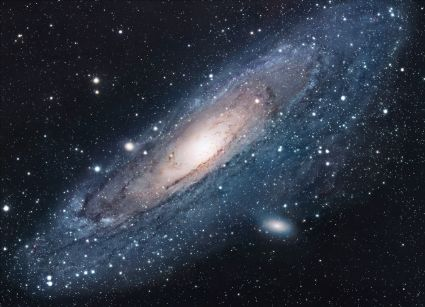
\includegraphics[scale=1.5]{images/universe.jpg}
    \caption{Image example.}
    \label{fig:my_label}
\end{figure}

\lipsum[2]

% ----------------------------------
\section*{Exercise 2}

\lipsum[1]

\begin{figure}[h!]
    \centering
    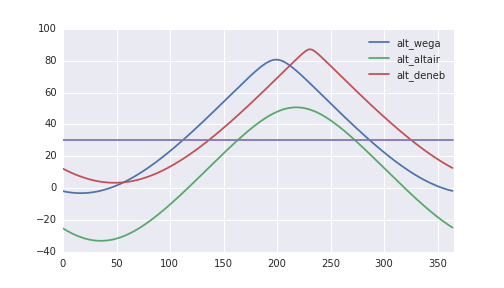
\includegraphics[width=0.65\linewidth]{images/diagram_1.png}
    \caption{Diagram example: all texts in the plot should be readable! \\ {\color{red}\textbf{No screenshots are allowed! \\ All figures must be saved as images and included into the final archive.}} }
    \label{fig:my_label}
\end{figure}


\begin{table}[h!]
    \centering
    \begin{tabular}{ |p{3cm}||p{3cm}|p{3cm}|p{3cm}|  }
     \hline
     \multicolumn{4}{|c|}{Country List} \\
     \hline
     Country Name     or Area Name& ISO ALPHA 2 Code &ISO ALPHA 3 Code&ISO numeric Code\\
     \hline
     Afghanistan   & AF    &AFG&   004\\
     Aland Islands&   AX  & ALA   &248\\
     Albania &AL & ALB&  008\\
     Algeria    &DZ & DZA&  012\\
     American Samoa&   AS  & ASM&016\\
     Andorra& AD  & AND   &020\\
     Angola& AO  & AGO&024\\
     \hline
    \end{tabular}
    \caption{Table example.}
    \label{tab:my_label}
\end{table}

\lipsum[3]

% -------------------------------
\newpage
\section*{Exercise 3}

\noindent \textbf{Example of adding a hand written notes.} \\
\textbf{ \color{red} Please, scan carefully your hand written text and insert it as an image.} \\
\textbf{ \color{red} The hand written text must be readable!} \\

\begin{figure}[h!]
    \centering
    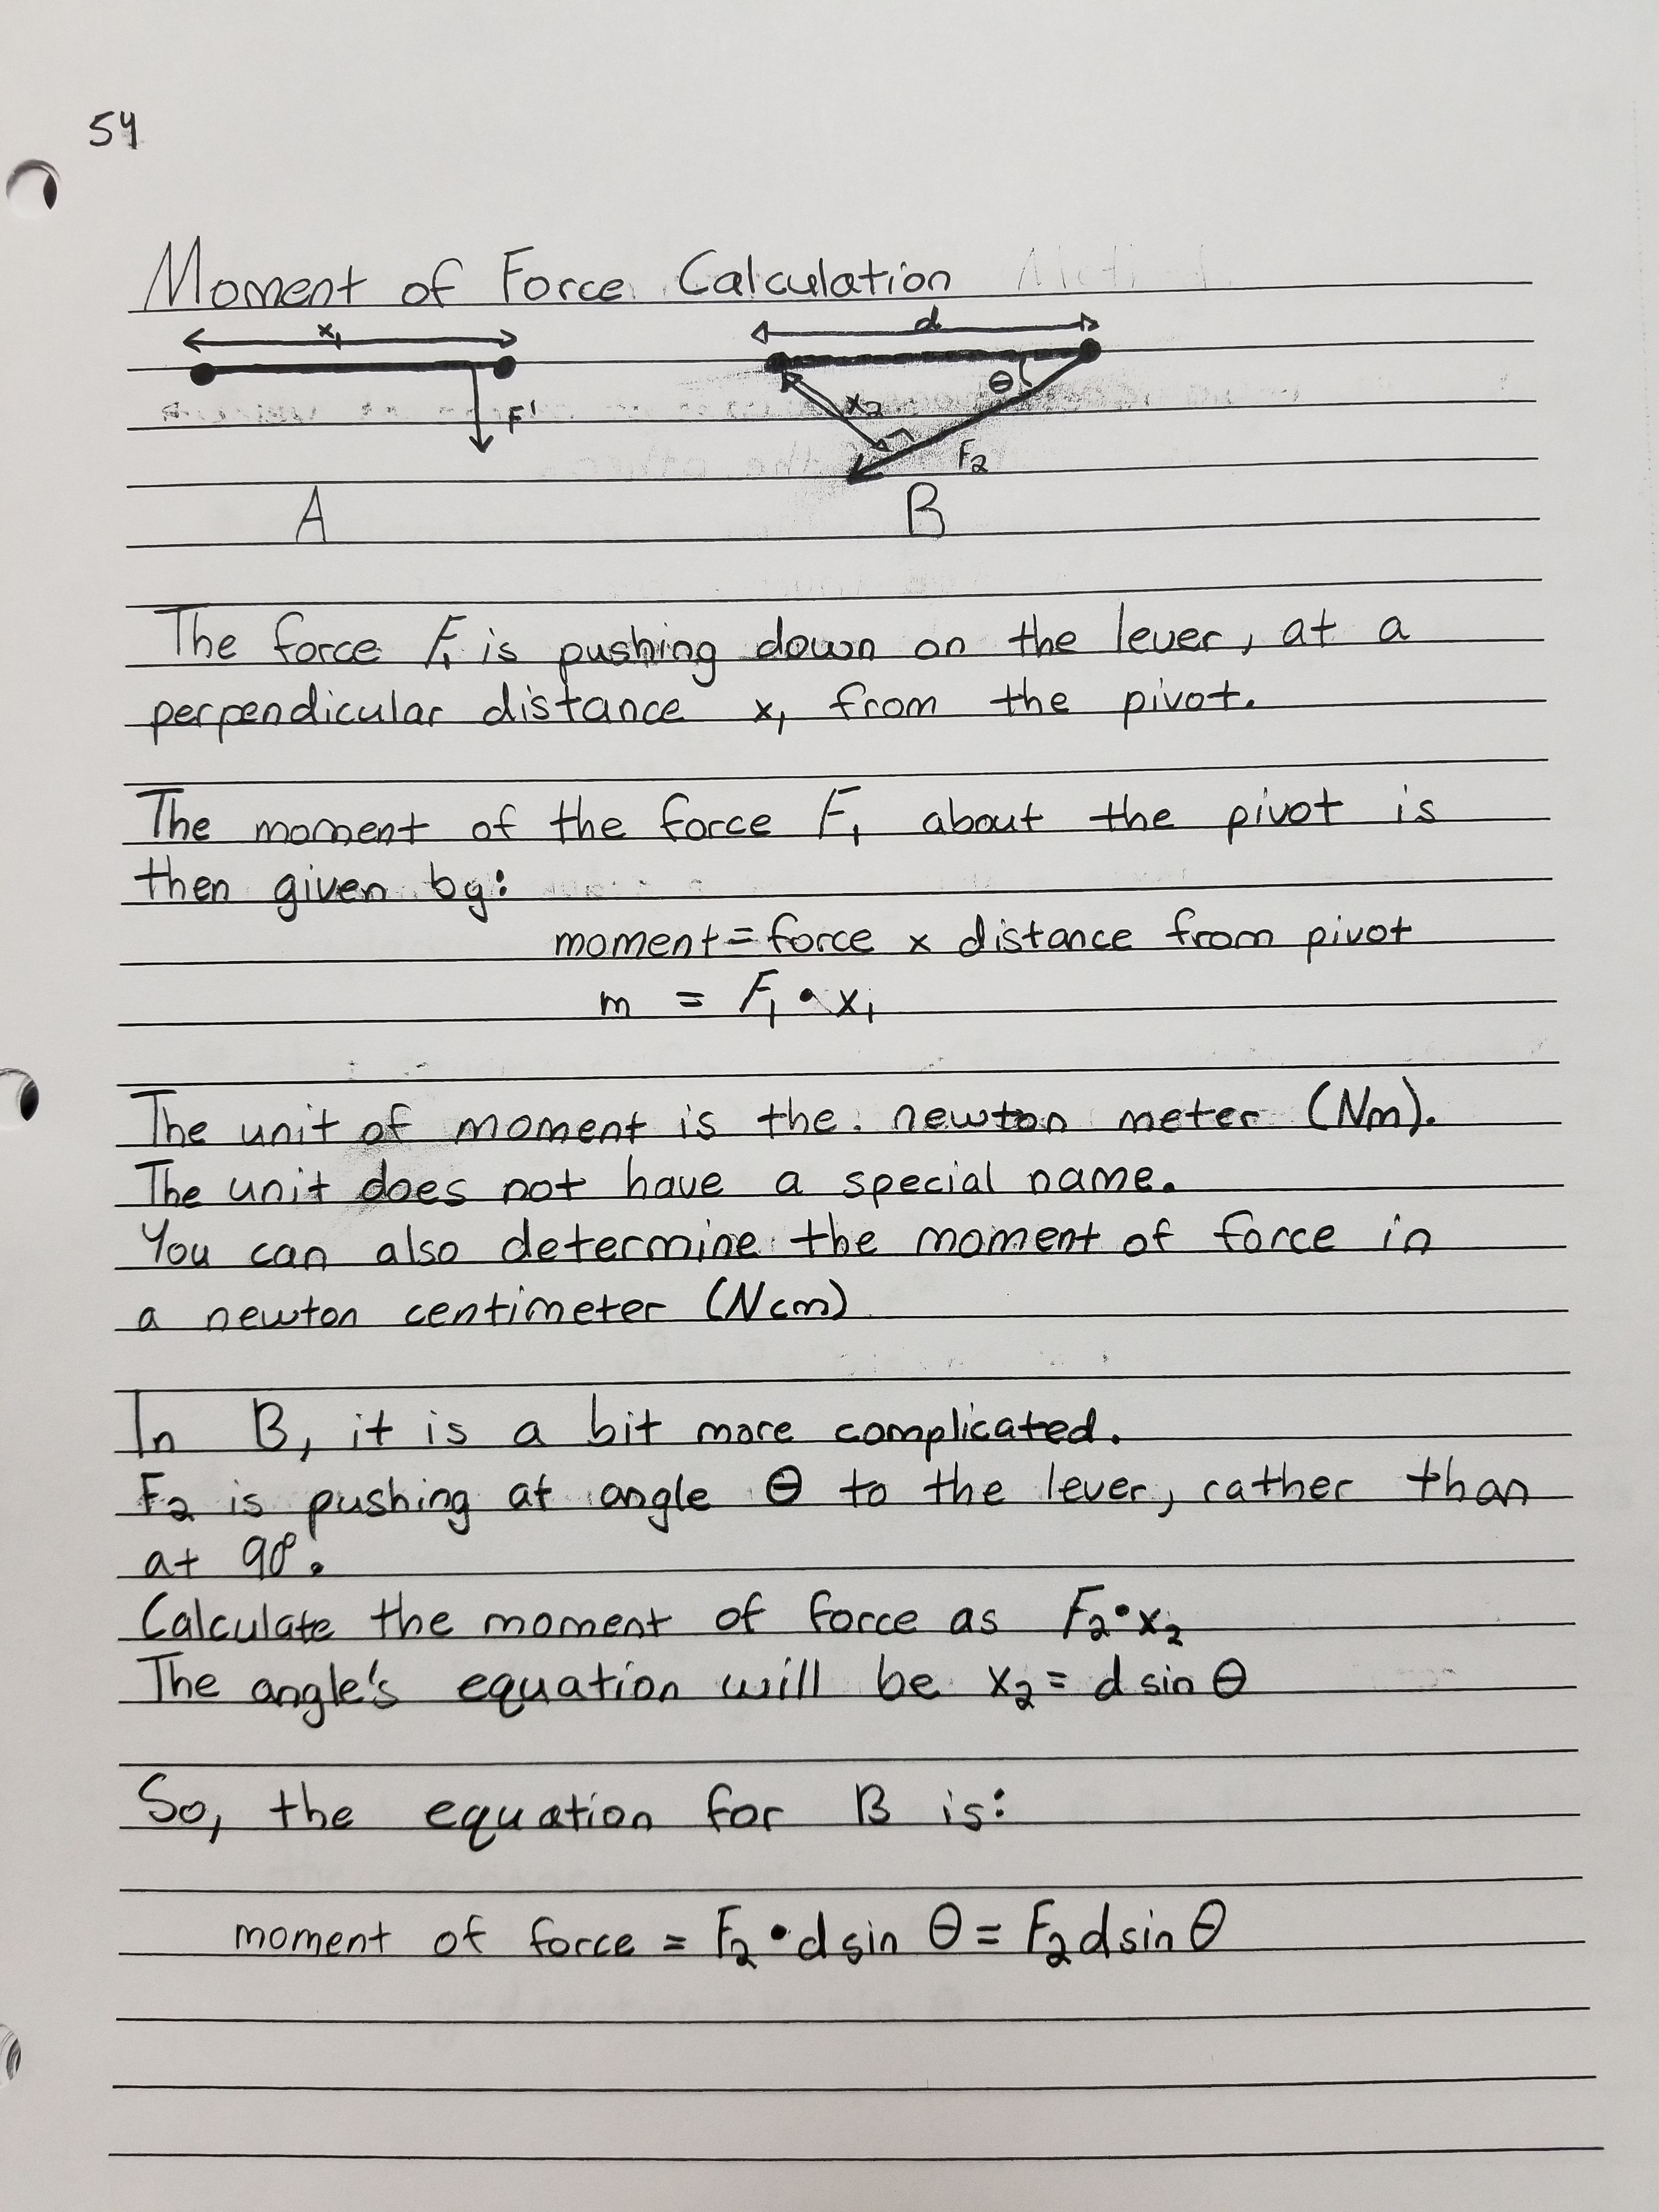
\includegraphics[width=0.96\linewidth]{images/hand_text.jpg}
\end{figure}

\section*{Exercise 4}

\lipsum[1]

\begin{equation*}
x_{1,2} = {{-b  \pm \sqrt{b^2 - 4ac}} \over 2a}
\end{equation*}

\begin{center}
    {\color{red}\textbf{Do not write formulas in plain text! \\
    a*x2 + b*x + c = 0 won't be accepted.}}
\end{center}

\lipsum[2]

\begin{equation}
    f(\vec{x}) =
    \begin{bmatrix}
    a_{1,1} & \cdots & a_{1,n} \\
    \vdots  & \ddots & \vdots  \\
    a_{m,1} & \cdots & a_{m,n} 
\end{bmatrix}
\cdot
\begin{bmatrix}
    x_{1} \\
    \vdots  \\
    x_{n} 
\end{bmatrix}
= \lambda \cdot \vec{x}
\end{equation}

\begin{center}
    {\color{red}\textbf{You may also use numeration for equations to easily refer to them in the text.}}
\end{center}


\end{document}
